% =============================================================================
% Replication report skeleton: Baland, Cassan & Decerf (2021), "Too Young to Die"
% Course: Development Economics 2026, Madras School of Economics
% Due: 17 Oct 2026 (Classroom -> "Replication Submission")
%
% WHAT THIS FILE IS: structure, equations, tables with our numbers, figures,
% and the facts each paragraph must cover. WHAT IT IS NOT: submission prose.
% The course's integrity rule says the team writes the report text; AI may only
% help with ideas, literature search, code and grammar. Every \todo{} marks
% text the team has to write in its own words. Delete every \todo before export.
%
% Build: xelatex main.tex  (twice).  Needs Times New Roman (Windows has it).
% Spec: TNR 12 pt, 1.5 spacing, 2.54 cm margins, page + section numbers.
% =============================================================================
\documentclass[12pt,a4paper]{article}
\usepackage[margin=2.54cm]{geometry}
\usepackage{fontspec}
\setmainfont{Times New Roman}
\usepackage{setspace}
\onehalfspacing
\usepackage{amsmath}
\usepackage{graphicx}
\usepackage{booktabs}
\usepackage{longtable}
\usepackage{array}
\usepackage{xcolor}
\usepackage[hidelinks]{hyperref}
\usepackage{float}
\usepackage{caption}
\captionsetup{font=small,labelfont=bf}
\setlength{\parindent}{0pt}
\setlength{\parskip}{0.5em}

\newcommand{\todo}[1]{\textbf{\textcolor{red}{[TEAM: #1]}}}
\newcommand{\ahat}{\hat{a}}
\graphicspath{{../../../development_economics/output/replication/figures/}}

\begin{document}

% ---------------------------------------------------------------- title page
\begin{titlepage}
\centering
\vspace*{3cm}
{\Large\bfseries Replication of ``Too Young to Die: Deprivation Measures Combining Poverty and Premature Mortality''\par}
\vspace{1cm}
{\large Baland, Cassan and Decerf (2021), \emph{American Economic Journal: Applied Economics}, 13(4), 226--257\par}
\vspace{2cm}
Development Economics 2026\\ Madras School of Economics\\[1em]
Replication submission, 17 October 2026\\[2em]
Ashwath, Drishti, Johan\\[0.5em]
Group leader: Drishti \todo{contact email and phone}
\end{titlepage}

\section{Introduction}
\todo{Write this section yourselves. Points it must cover, with sources:}
\begin{itemize}
  \item Puzzle: Botswana 1990--2000. Extreme poverty 33.6\% $\to$ 29.5\%, life expectancy 63.6 $\to$ 45.6 years (paper p.\,226). Did total deprivation fall?
  \item Gap in existing measures: head-count ratio (HC) counts only the living. A poor person who dies leaves the denominator, so HC can fall because the poor die (the ``mortality paradox'', p.\,231 fn 7).
  \item Contribution: dying before an age threshold $\ahat$ is a deprivation of its own (life-span deprivation). Person-years prematurely lost (PYPL) are added to person-years in alive deprivation (PYAD), then divided by one reference population. Two indexes: Inherited Deprivation (ID) and Generated Deprivation (GD).
  \item Theoretical mechanism to state explicitly (the rubric asks for it): premature death is exclusive of poverty (the dead cannot be poor), so the two deprivations add in time units. A single reference population removes the inconsistency of composite indexes (Table~1 below).
  \item Headline results to be replicated: ignoring mortality understates world deprivation by 27\% (1990) to 36\% (2015); GD and HC give opposite trend verdicts in 8.4\% of five-year comparisons.
  \item What this report does: reproduces every table and figure except Figure~1 (a schematic), from the authors' public package, and explains each gap.
  \item Roadmap sentence.
\end{itemize}

\section{Data}
\todo{Write the data section. Facts to cover:}
\begin{itemize}
  \item \textbf{Mortality and population:} Global Burden of Disease 2017 round (GBD Collaborative Network, 2018). All-cause deaths and rates per 100,000, both sexes, by age group, country and year, 1990--2017. Point estimates only; 5-year age bins except 0--1 and 1--4.
  \item \textbf{Alive deprivation:} PovCalNet (World Bank, 2019). Head-count ratio at \$1.90 per day (2011 PPP). Survey-based, three-yearly, \emph{linearly interpolated} to annual values (Chen \& Ravallion, 2013).
  \item \textbf{Regions:} World Bank classification file.
  \item \textbf{Sample:} 113 low- and middle-income countries, 1990--2015, plus six regions and the World. A country enters only with an HC value in every year. The sample is 113 because the authors' name-based merge drops Eswatini (``Swaziland'' in GBD) and West Bank and Gaza (``Palestine''), and Kiribati sits in their drop list; an ISO3 merge gives 116.
  \item \textbf{Vintage:} we use the exact files in the authors' openICPSR package (E119941V1), so no data revision enters. PovCalNet has since been retired (succeeded by PIP); later GBD rounds revise history.
  \item \textbf{France (Figure~5):} Human Mortality Database. \textbf{Not yet re-run from the shared repository} (files pending); see Section~\ref{sec:gaps}.
\end{itemize}

\section{Methodology}
\todo{Explain the two indexes in your own words. Equations and notation below are from the paper (pp.\,232--234) and can be used as they stand.}

Notation: $t$ is the year; $\ahat$ the life-span threshold; $f$, $p$ the numbers alive non-poor and alive poor; $d$ the number prematurely dead; $n_a$ the number alive at age $a$; $\mu_a$ age-specific mortality; $\gamma>0$ the weight of one PYPL relative to one PYAD.

\begin{align}
ID_\gamma(x) &= \frac{p(x)}{f(x)+p(x)+d(x)} + \gamma\,\frac{d(x)}{f(x)+p(x)+d(x)} \label{eq:id}\\[0.3em]
GD_\gamma(x,\mu) &= \frac{p(x)}{f(x)+p(x)+d^{GD}(x,\mu)} + \gamma\,\frac{d^{GD}(x,\mu)}{f(x)+p(x)+d^{GD}(x,\mu)} \label{eq:gd}\\[0.3em]
d^{GD}(x,\mu) &= \sum_{a=0}^{\ahat-1} n_a(x)\,\mu_a\,\bigl(\ahat-(a+1)\bigr) \label{eq:dgd}
\end{align}

Things the methodology section must state:
\begin{itemize}
  \item Baseline parameters: $\ahat=50$, $\gamma=1$, poverty line \$1.90. Other thresholds used: $\ahat=5$ (Haiti, Figure~3), $40$ (France, Figure~5), $80$ (sensitivity, p.\,251).
  \item \textbf{Timing convention.} Equation~\eqref{eq:dgd} books deaths at the end of the period (loss of $\ahat-(a+1)$ years). The authors' empirical code books them at the start (loss of $\ahat-a$ years), consistent with their footnote~3. Our empirical results use $\ahat-a$. The theory figures (Figures~2 and 4) use equation~\eqref{eq:dgd} as printed.
  \item Only GD is estimated for the world, because ID needs $\ahat$ years of past deaths by age. ID is computed only for Haiti (Figure~3) and France (Figure~5).
  \item How the code builds the panel: population at the start of the year $=$ deaths $\div$ (rate $/100{,}000$), truncated; ``living population'' is the end-of-year population (start minus deaths); 5-year bins are split into single ages assuming a constant death rate within a bin and geometrically declining cohort sizes; everyone in 95+ dies that year; regional and World aggregates sum deaths and population by age bin before the same split; HC is aggregated with population weights.
  \item Ranks and reversals: ranks ascending within a year (least deprived $=1$); average $|{\rm rank}_{GD}-{\rm rank}_{HC}|$; a reversal is a country-year where $GD_t/GD_{t-5}$ and $HC_t/HC_{t-5}$ lie on opposite sides of 1.
  \item Software and workflow: Stata, written independently of the authors' do-files, then checked against the authors' own code run on the same raw data.
\end{itemize}

\section{Replication}
\todo{Introduce each result in one or two sentences of your own, say whether it matches, and point to Section~\ref{sec:gaps} for gaps.}

\subsection{Theory examples (no data)}

\begin{table}[H]
\centering
\caption*{\textbf{Table 1.} The composite index $P_{0.5}$ is inconsistent (paper p.\,228)}
\begin{tabular}{lccc}
\toprule
 & Society A & Society B & Society C\\
\midrule
Head-count ratio (HC) & 0.50 & 0.33 & 0.00\\
Share of young dead (LD) & 0.00 & 0.25 & 0.50\\
Composite $P_{0.5}$ & 0.25 & 0.29 & 0.25\\
\bottomrule
\end{tabular}

\smallskip
{\small Source: our computation (\texttt{09\_simulations.do}); matches the paper.}
\end{table}

\begin{table}[H]
\centering
\caption*{\textbf{Table 2.} HC against ID on distributions $x$, $x'$, $x''$ (paper p.\,231)}
\begin{tabular}{lccc}
\toprule
 & $x$ & $x'$ & $x''$\\
\midrule
HC & 0 & 0 & 0.5\\
$ID_1$ & 0.5 & 0 & 0.5\\
$ID_2$ & 1.0 & 0 & 0.5\\
\bottomrule
\end{tabular}

\smallskip
{\small Source: our computation (\texttt{09\_simulations.do}).}
\end{table}

\begin{figure}[H]
\centering
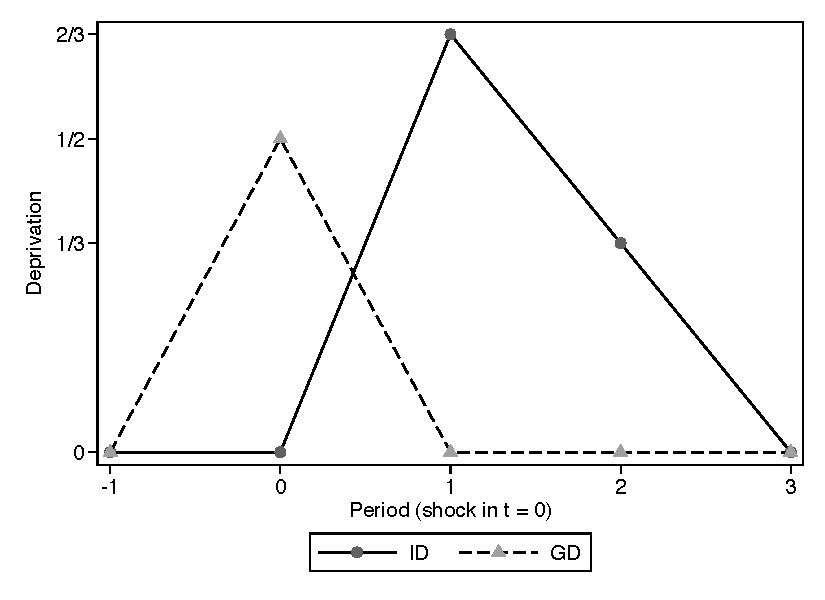
\includegraphics[width=0.8\textwidth]{fig02_transitory_shock.pdf}
\caption*{\textbf{Figure 2.} Response of ID and GD to a transitory shock. Source: our simulation.}
\end{figure}

\begin{figure}[H]
\centering
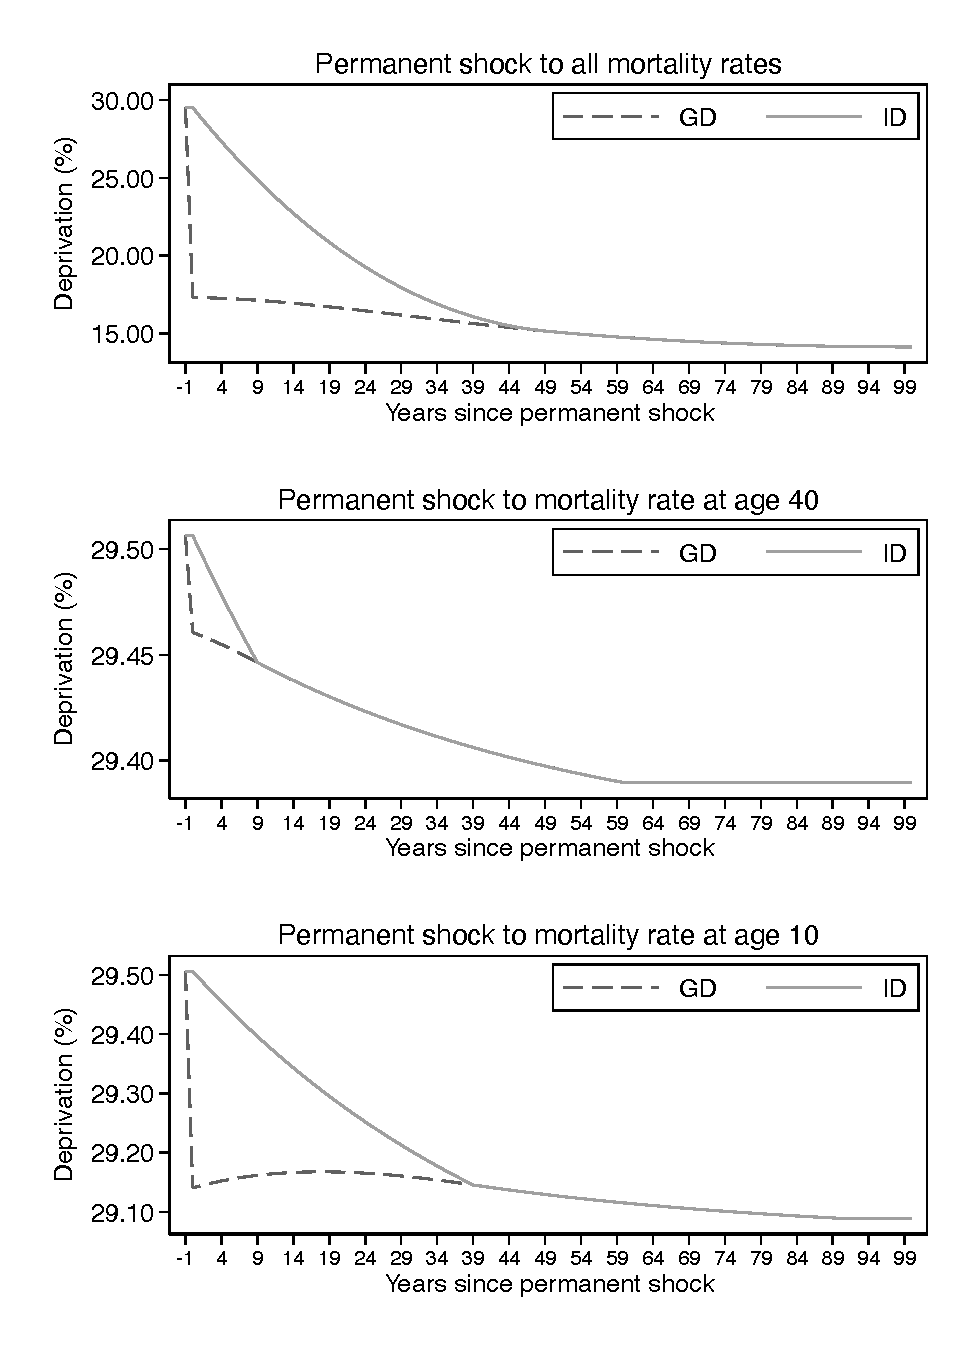
\includegraphics[width=0.8\textwidth]{fig04_permanent_shocks.pdf}
\caption*{\textbf{Figure 4.} Response of ID and GD to permanent mortality shocks ($\ahat=50$). Source: our simulation; identical to the authors' Excel sheet.}
\end{figure}

\subsection{Worldwide deprivation}

\begin{table}[H]
\centering
\caption*{\textbf{Table 3.} World Generated Deprivation, $\ahat=50$, $\gamma=1$ (person-years in millions unless stated)}
\small
\begin{tabular}{lrrrr}
\toprule
 & \multicolumn{2}{c}{1990} & \multicolumn{2}{c}{2015}\\
\cmidrule(lr){2-3}\cmidrule(lr){4-5}
 & Paper & Ours & Paper & Ours\\
\midrule
Living population & 4,200 & 4,197.9 & 6,010 & 6,007.0\\
Head-count ratio (\%) & 44.9 & 44.87 & 11.7 & 11.74\\
Alive deprivation (PYAD) & 1,886 & 1,883.7 & 703 & 705.2\\
Life-span deprivation (PYPL) & 701 & 701.4 & 402 & 402.4\\
Deprived population & 2,587 & 2,585.1 & 1,105 & 1,107.6\\
Reference population & 4,901 & 4,899.3 & 6,412 & 6,409.4\\
$GD_1$ (\%) & 52.8 & 52.76 & 17.2 & 17.28\\
\bottomrule
\end{tabular}

\smallskip
{\small Source: our computation (\texttt{10\_tables.do}). The paper's cells are hand-computed from rounded rows (see Section~\ref{sec:gaps}).}
\end{table}

\begin{figure}[H]
\centering
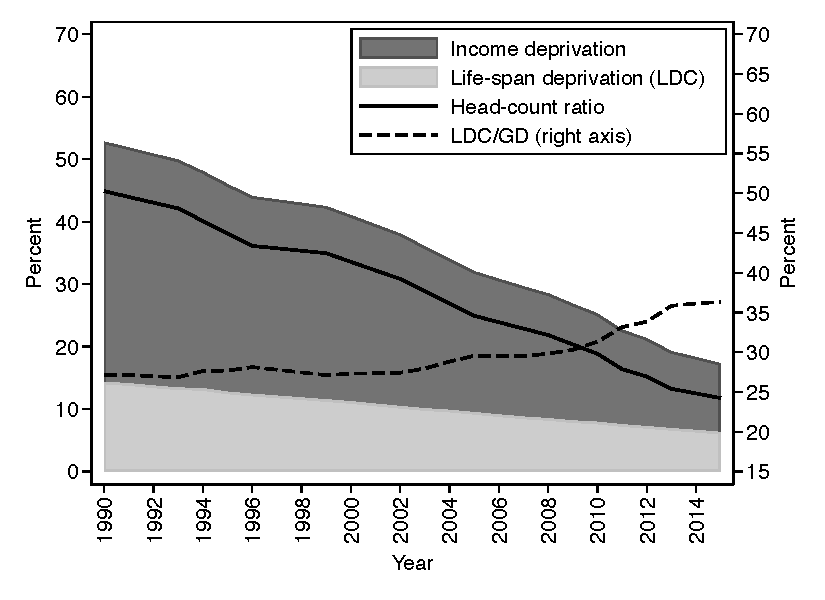
\includegraphics[width=0.85\textwidth]{fig06_world_decomposition.pdf}
\caption*{\textbf{Figure 6.} World deprivation: income and life-span components of GD, head-count ratio, and life-span share, 1990--2015. Source: our computation.}
\end{figure}

\begin{figure}[H]
\centering
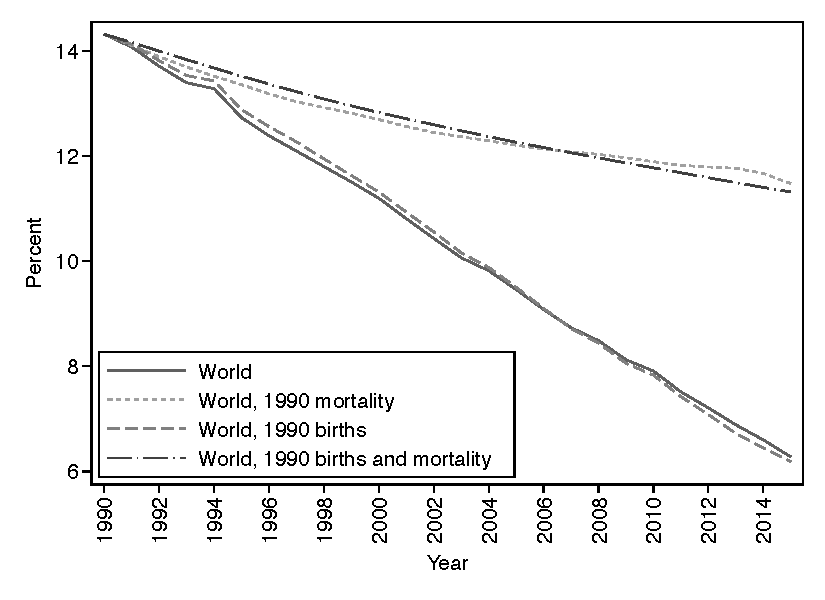
\includegraphics[width=0.85\textwidth]{fig07_counterfactuals.pdf}
\caption*{\textbf{Figure 7.} Life-span component of GD with 1990 births, 1990 mortality, or both held fixed. Source: our computation.}
\end{figure}

\todo{Say in your own words what Table 3 and Figures 6--7 show. Numbers to use: life-span share rose from 27.1\% to 36.3\%; at $\ahat=80$ the 2015 share is 60.4\%; under-5 deaths are 79\% (1990) and 68\% (2015) of PYPL; natality does not drive the fall (births +3.3\%), mortality decline and pyramid composition do.}

\subsection{Countries}

\begin{table}[H]
\centering
\caption*{\textbf{Table 4.} Gabon and Morocco, 1993 (person-years in thousands unless stated)}
\small
\begin{tabular}{lrrrr}
\toprule
 & \multicolumn{2}{c}{Gabon} & \multicolumn{2}{c}{Morocco}\\
\cmidrule(lr){2-3}\cmidrule(lr){4-5}
 & Paper & Ours & Paper & Ours\\
\midrule
Living population & 1,043 & 1,043.8 & 26,449 & 26,449.0\\
Head-count ratio (\%) & 5.2 & 5.17 & 5.8 & 5.78\\
Alive deprivation (PYAD) & 54 & 53.9 & 1,534 & 1,527.5\\
Life-span deprivation (PYPL) & 174 & 173.9 & 3,100 & 3,100.3\\
Deprived population & 228 & 227.8 & 4,634 & 4,627.8\\
Reference population & 1,217 & 1,217.6 & 29,549 & 29,549.3\\
$GD_1$ (\%) & \textbf{17.9} & \textbf{18.71} & 15.7 & 15.66\\
\bottomrule
\end{tabular}

\smallskip
{\small Source: our computation (\texttt{10\_tables.do}). Gabon's published $GD_1$ divides by 1,271 instead of 1,217.}
\end{table}

\begin{figure}[H]
\centering
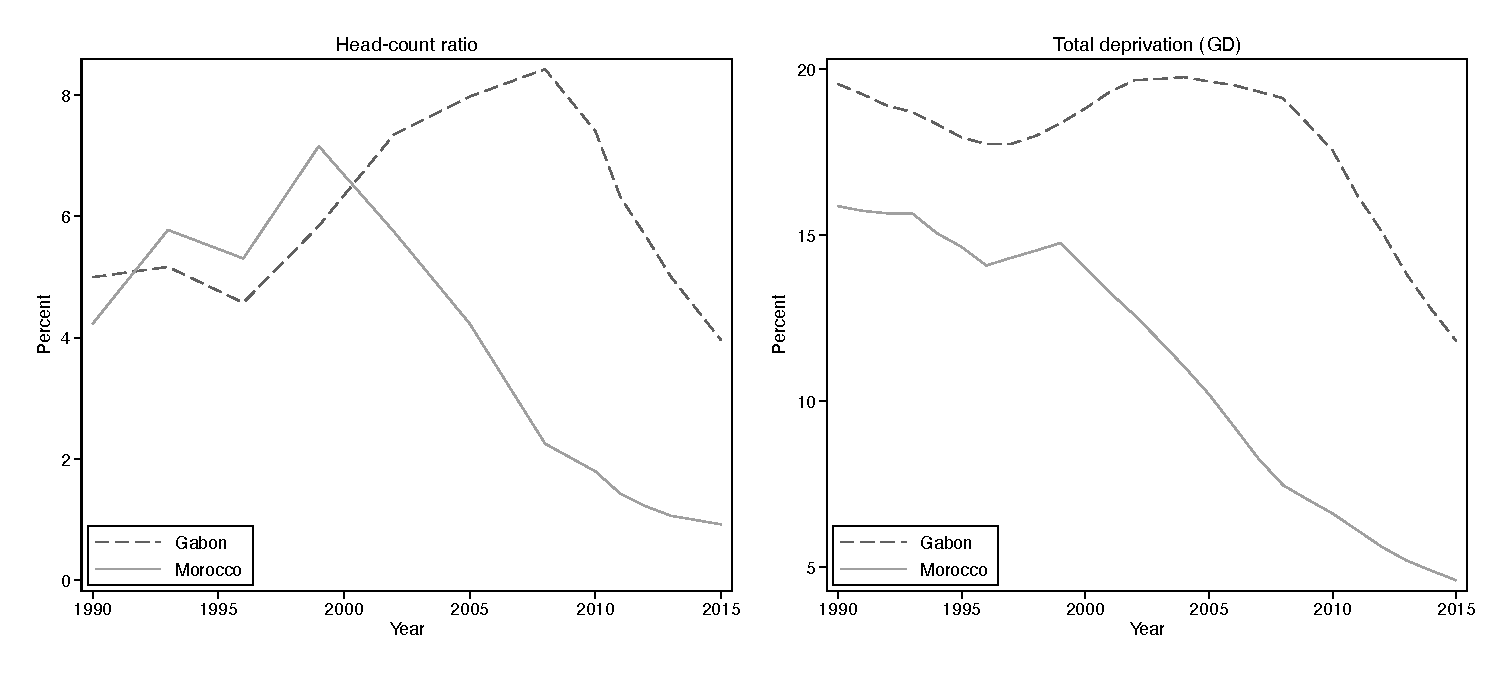
\includegraphics[width=0.9\textwidth]{fig08_gabon_morocco.pdf}
\caption*{\textbf{Figure 8.} Gabon and Morocco: head-count ratio (left) and GD (right). Source: our computation.}
\end{figure}

\begin{figure}[H]
\centering
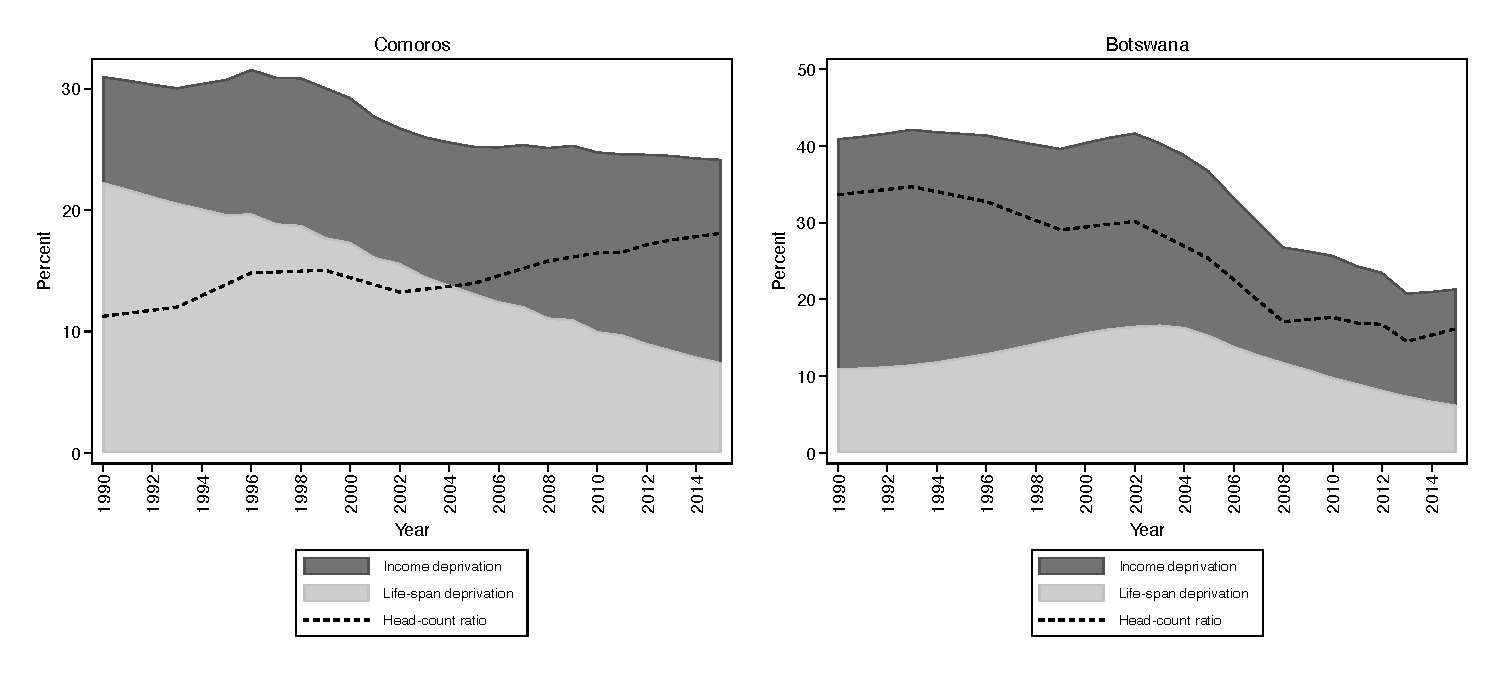
\includegraphics[width=0.9\textwidth]{fig09_comoros_botswana.pdf}
\caption*{\textbf{Figure 9.} Comoros and Botswana: GD and HC, stacked. Source: our computation.}
\end{figure}

\begin{figure}[H]
\centering
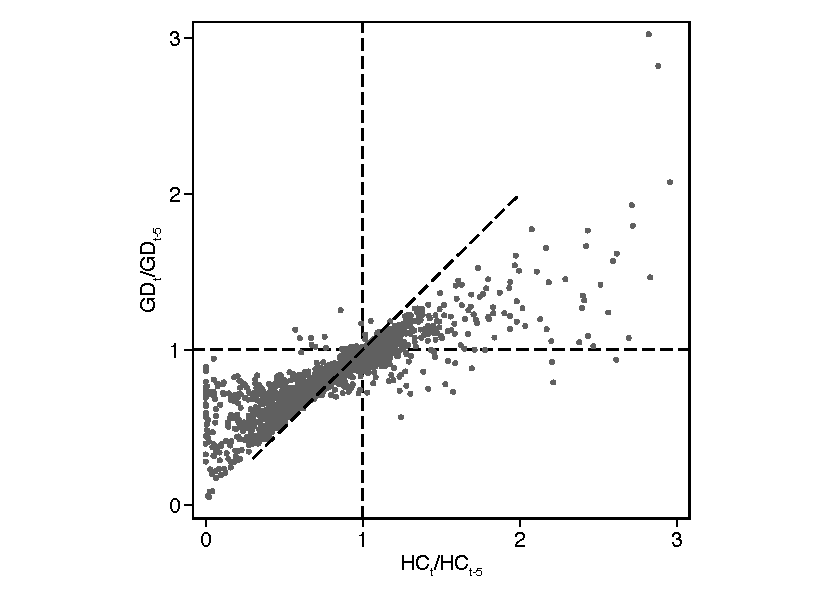
\includegraphics[width=0.7\textwidth]{fig10_trend_reversals.pdf}
\caption*{\textbf{Figure 10.} Five-year change in GD against five-year change in HC (HC ratio below 3). Source: our computation.}
\end{figure}

\todo{Say in your own words what Table 4 and Figures 8--10 show. Numbers to use: Gabon moves from rank 19 (HC) to 38 (GD), Morocco from 21 to 32 (113 countries, 1993); average rank change 4.1; Comoros HC +60.9\% while GD $-22.0$\%; Botswana HC $-11.4$\% while GD $+0.5$\% over 1990--2001; reversals 8.4\% ($\gamma=1$) and 26.9\% ($\gamma\to\infty$).}

\subsection{Haiti and France}

\begin{figure}[H]
\centering
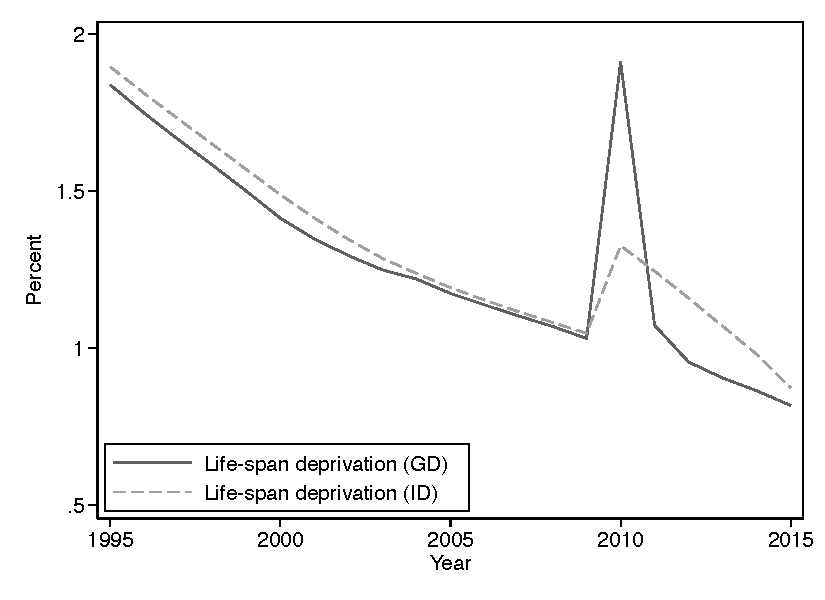
\includegraphics[width=0.85\textwidth]{fig03_haiti.pdf}
\caption*{\textbf{Figure 3.} Haiti: life-span components of ID and GD, $\ahat=5$, 1995--2015. Source: our computation.}
\end{figure}

\begin{figure}[H]
\centering
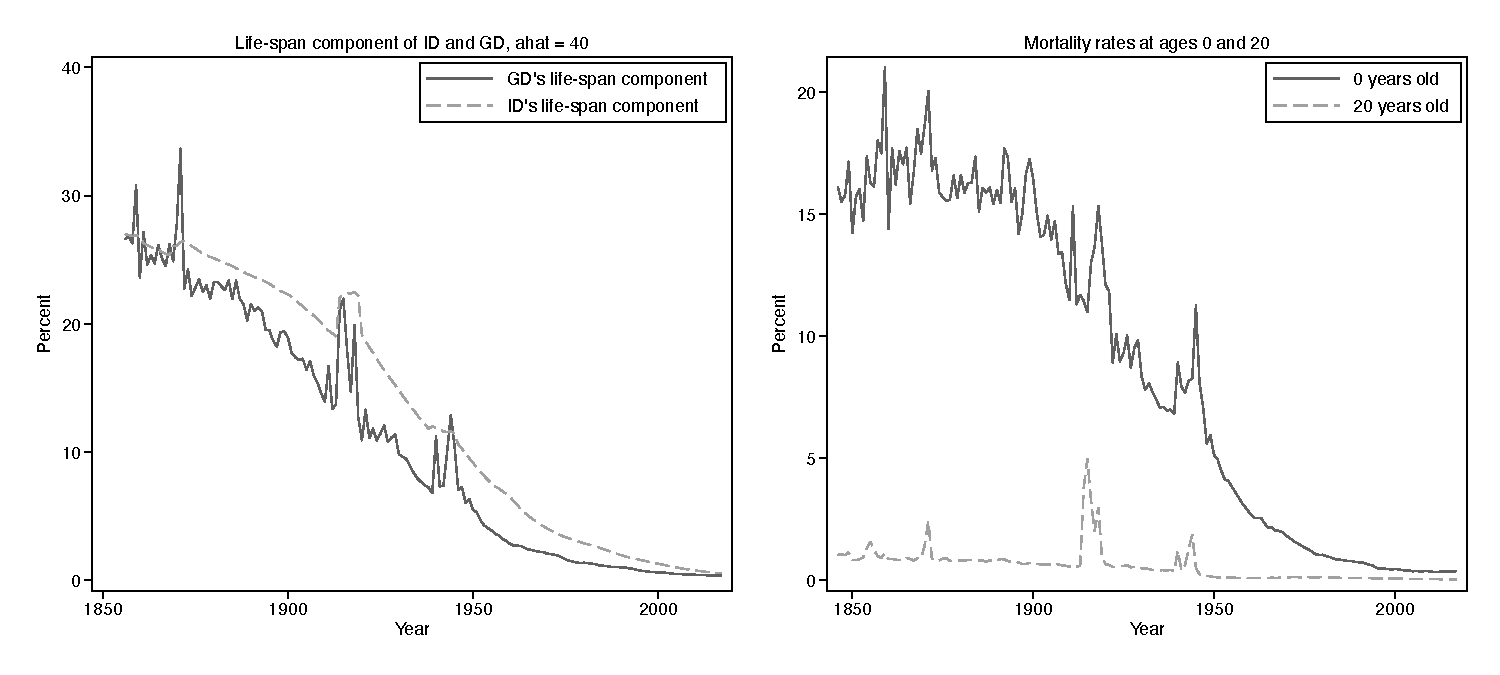
\includegraphics[width=\textwidth]{fig05_france.pdf}
\caption*{\textbf{Figure 5.} France: life-span components of ID and GD ($\ahat=40$) and mortality at ages 0 and 20. Source: our computation from HMD period life tables (2026 vintage).}
\end{figure}

\todo{Figure 5 caveat: the HMD files were downloaded on 11 Oct 2026 by a teammate and are not in the shared repository. Do not describe Figure 5 as verified until the files are re-run (see audit note).}

\section{Where our results differ from the published paper}\label{sec:gaps}
\todo{Write this section in your own words; the rubric gives marks for explaining divergences. The table below lists every checked quantity that does not match, what the authors' own code gives, and the status. ``Verified'' means confirmed by running the authors' Stata code on their raw data.}

\begin{longtable}{>{\raggedright}p{3.4cm}>{\raggedright}p{1.6cm}>{\raggedright}p{1.7cm}>{\raggedright}p{2cm}>{\raggedright\arraybackslash}p{5.2cm}}
\caption*{\textbf{Table 5.} Published numbers that do not match, and what explains them}\\
\toprule
Item & Paper & Ours & Authors' code & Status\\
\midrule
\endfirsthead
\toprule
Item & Paper & Ours & Authors' code & Status\\
\midrule
\endhead
Gabon $GD_1$, Table 4 (\%) & 17.9 & 18.71 & 18.71 & Verified. Their do-file computes $228/1271$ (a typo for 1217); the correct value is 18.7.\\
Average rank change, 1990 & 4.4 & 4.92 & 4.92 & Verified. The paper's 1990 and 2015 values are swapped.\\
Average rank change, 2015 & 4.9 & 4.39 & 4.34 & Verified. Same swap. Our value differs from the authors' only through tie-breaking among countries with HC at or near zero.\\
Comoros HC change 1990--2015 (\%) & +60 & +60.9 & same as ours & Within rounding.\\
Comoros GD change 1990--2015 (\%) & $-23$ & $-22.0$ & same as ours & Unexplained. No start or end year in 1990--2015 gives $-23$.\\
Botswana HC change 1990--2001 (\%) & $-12$ & $-11.4$ & same as ours & Sensitive to end year ($-12.5$ for 2000). Unexplained.\\
Botswana GD change 1990--2001 (\%) & +0.7 & +0.5 & same as ours & No end year gives both published values. Unexplained.\\
Botswana HC in 2000 (\%) & 29.5 & 29.43 & same as ours & Possibly the PovCalNet interpolation. Unexplained.\\
Newborn mortality 1990 and 2015 (\%) & 6.6, 3.4 & 6.76, 3.47 & not computed & Definition not in the authors' code. Small gap.\\
Births, 1990--2015 (\%) & +2.8 & +3.3 & not computed & Same.\\
Median age at death & 64 & 58 (pooled), 65 (2015) & not computed & Possibly a comparison of different periods: the yearly median is 64--65 in 2012--2015. To be confirmed.\\
\bottomrule
\end{longtable}

Further points the section should cover:
\begin{itemize}
  \item \textbf{Rounding in the paper's Tables 3 and 4.} The authors' do-file builds those cells by hand from rounded rows (e.g.\ \texttt{di 26449*0.058} gives 1,534 for Morocco's PYAD, while the code's own value is 1,527.5). Applying the same rounding to our numbers reproduces every cell. Examples: the introduction's 705 million poor in 2015 is correct, and Table 3's 703 is $6{,}010\times0.117$.
  \item \textbf{Timing convention:} equation~\eqref{eq:dgd} ($\ahat-(a+1)$) against the code ($\ahat-a$). Resolved: use $\ahat-a$ for the empirics.
  \item \textbf{Sample:} 113 against 116 countries (Eswatini, West Bank and Gaza, Kiribati).
  \item \textbf{Ranks near the top of the table} are not robust: four countries have HC $=0$ in 2015 and ten have HC $<0.1\%$, so rank statistics depend on the tie rule. Azerbaijan's loss is 26 ranks in 2010 and 2014 under our rule; in the authors' output the maximum is 26 in 2008 and 25 in 2014.
  \item \textbf{Figure 5:} the package readme asks for cohort life tables, but the figure can only come from period tables (cohort tables stop at the 1933 cohort). The Alsace-Lorraine fall in ID appears in 1920 with 2026 HMD data, in 1919 in the paper. \todo{State as unverified until the HMD files are re-run.}
  \item \textbf{What matches exactly:} Table 3 (to rounding), life-span shares 27.1\% and 36.3\%, 60.4\% at $\ahat=80$, 113 countries, Gabon and Morocco ranks (19 $\to$ 38, 21 $\to$ 32), reversals 8.42\% and 26.88\%, Botswana HC in 1990 (33.6\%), Figure 4 against the authors' Excel.
\end{itemize}

\section{Conclusion}
\todo{Short conclusion: what replicated, what did not and why, and one sentence on the extension direction once the team has chosen it.}

\section*{Contribution of each member}
\todo{Who did what (required in the final submission; keep a draft here).}

\section*{AI-use declaration}
\todo{Declare, in the course's categories, what AI was used for. The AI-use log in the unit README lists what has been done so far.}

\section*{References}
\hangindent=0.5in\noindent Baland, J.-M., Cassan, G., \& Decerf, B. (2021). ``Too young to die'': Deprivation measures combining poverty and premature mortality. \emph{American Economic Journal: Applied Economics, 13}(4), 226--257. https://doi.org/10.1257/app.20200122

\hangindent=0.5in\noindent Baland, J.-M., Cassan, G., \& Decerf, B. (2021). \emph{Replication data for: ``Too young to die''} [Data set]. openICPSR. https://doi.org/10.3886/E119941V1

\hangindent=0.5in\noindent Chen, S., \& Ravallion, M. (2013). More relatively-poor people in a less absolutely-poor world. \emph{Review of Income and Wealth, 59}(1), 1--28. \todo{verify against the source}

\hangindent=0.5in\noindent GBD 2017 Collaborative Network. (2018). \emph{Global Burden of Disease Study 2017 (GBD 2017) results}. Institute for Health Metrics and Evaluation. \todo{add URL and access date}

\hangindent=0.5in\noindent World Bank. (2019). \emph{PovcalNet} [Database]. Development Research Group. \todo{add URL and access date}

\end{document}
